\documentclass[a4paper, 12pt]{article}
\usepackage{amssymb}
\usepackage{amsmath}
\usepackage{tikz}
\usepackage{multicol}
\usepackage{graphicx}
\graphicspath{ {./images/} }

\begin{document}

\title{Physics Beyond - Motion}
\author{Nathan Morris}
\maketitle

\newpage

\pagenumbering{roman}
\tableofcontents
\pagenumbering{arabic}

\newpage

\section{Procedure}
\begin{enumerate}
\item Define your problem
\item Model your problem mathematically. If the problem is about understanding the physics of something then:
\begin{itemize}
\item Model the description of that something (e.g. model what motion is)
\item Or investigate / find the underlying cause of that something (e.g. what causes motion)
\end{itemize}
\item Solve the maths
\item Interpret the results
\item (If needed) revise your model
\end{enumerate}

\newpage

\section{Definition:}
Definition - change in position (space) over time (time).
\begin{enumerate}
\item Put the physics of space time aside
\item Simple models - based on direct experience
\begin{itemize}
\item Space: Euclidean geometry
\item Time: Real numbers   
$\mathbb{R}$
\end{itemize}
\end{enumerate}

\section{Modelling Mathematically:}

\subsection{Q: What is the \underline{convenient} mathematical model?}
\begin{center}
\begin{tabular}{cc}
Function & Time $\rightarrow$ space\\
x: & $\mathbb{R}$ $\rightarrow$ space\\
& t $\mapsto$ position x(t)
\end{tabular}
\end{center}

\subsection{How to model space conveniently?}
$\rightsquigarrow$ need a reference frame.
\begin{center}
(0, $\vec{e_1}$, $\vec{e_2}$, $\vec{e_3}$)\\
$\vec{x}$ : $\mathbb{R}$ $\rightarrow$ Euclidean vector-space (after introducing 0)\\
$\vec{x}$ : $\mathbb{R}$ $\rightarrow$ $\mathbb{R}$$^3$\\
t $\mapsto$ $\vec{x}$(t) = 
$\begin{bmatrix}
x_1(t)\\ 
x_2(t)\\ 
x_3(t)\\ 
\end{bmatrix}$
\item (after introducing
$\begin{bmatrix}
\vec{e_1}, \vec{e_2}, \vec{e_3}\\
\end{bmatrix}$
\item Each $x_i$ : $\mathbb{R}$ $\rightarrow$$\mathbb{R}$ is ordinary an ordinary function we are familiar with
\centering
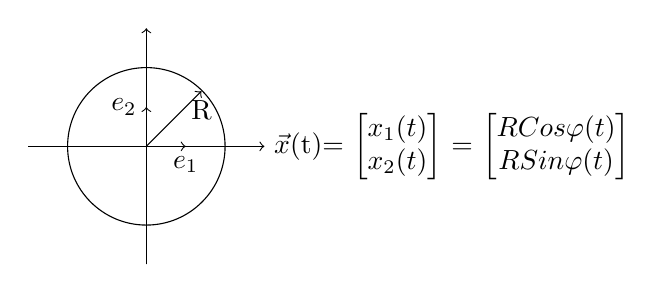
\begin{tikzpicture}
\draw[->] (-1.5,0) -- (0.5,0) node[below] {$e_1$};
\draw[->] (-1.5,0) -- (1.5,0) node[right] {$\vec{x}$(t)=
$\begin{bmatrix}
x_1(t)\\
x_2(t)\\
\end{bmatrix}$ = 
$\begin{bmatrix}
R Cos\varphi(t)\\
R Sin\varphi(t)\\
\end{bmatrix}$};
\draw[->] (0,-1.5) -- (0,0.5) node[left] {$e_2$};
\draw[->] (0,-1.5) -- (0,1.5);
\draw (0,0) circle (1cm);
\draw[->]  (0,0) -- (0.7,0.7) node[below] {R};
\end{tikzpicture}
\end{center}
Observation: interactions change motion.(This is how we detect interactions after all)

\subsection{Q: How to model changes in motion?}
************************Particle Motion Simulation**************************\\
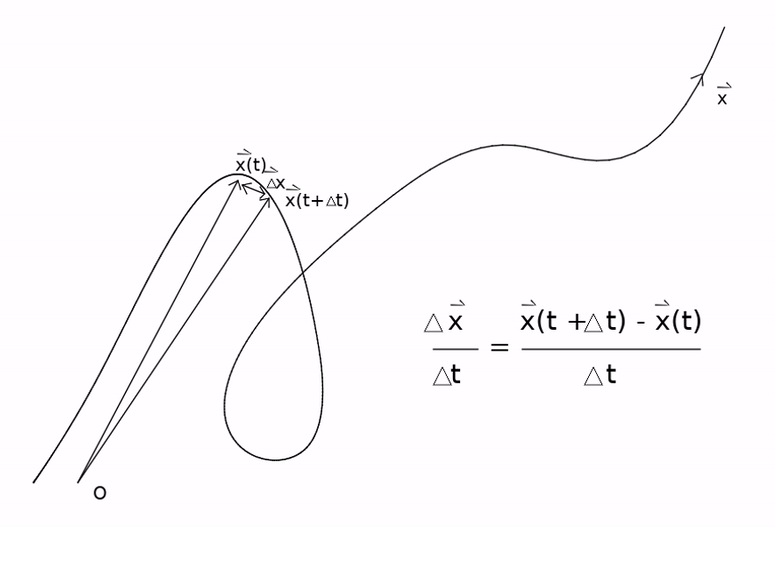
\includegraphics[scale=0.7]{Particle Motion Simulation}\\
\underline{Problem:} I need to find the velocity at one \underline{instant in time.}

\section{Q: How to model this mathematically}
$\rightarrow$ taking a limit:\\
$\vec{v}(t) = \displaystyle\lim_{\Delta t\to 0} \frac{\vec{x}(t+\Delta t) - \vec{x}(t)}{\Delta t}$\\
$\rightarrow$ or using infinitesimals

\section{The theory of infinitesimals}
\underline{Problem:} Define rates of change at \underline{one instant} in time.\\
The problem is that $\vec{v}$ is the \underline{average} velocity in the time interval [$t_0,t_0+\Delta t$]\\

\section{Q: How can we define \underline{instantaneous velocity}?}
\begin{enumerate}
\item The idea of a \underline{limit:}
\begin{itemize}
\item[-] make $\Delta$t smaller and smaller
\item[-] study $\frac{\Delta\vec{x}}{\Delta t}$ changes when $\Delta t$approaches 0   \end{itemize}
$\rightsquigarrow$ it becomes a tangent to the curve at $\vec{x}(t_0)$\\
we write:
\begin{center}
$\vec{v} = \frac{d \vec{x}}{dt} = \dot{\vec{x}} = \displaystyle\lim_{\Delta t\to 0} \frac{\vec{x}(t_0+\Delta t) - \vec{x}(t_0)}{\Delta t}$\\
\end{center}
Q: How is $\displaystyle\lim_{\Delta t \to 0}$ defined mathematically?\\
$\rightarrow$ it is technical and complicated
\item Idea of \underline{infinitesimals:}\\
\underline{Intuition}: If I zoom in onto a curve infinitely close, it becomes a \underline{straight line}.\\
************************Infinitesimals Simulation**************************\\
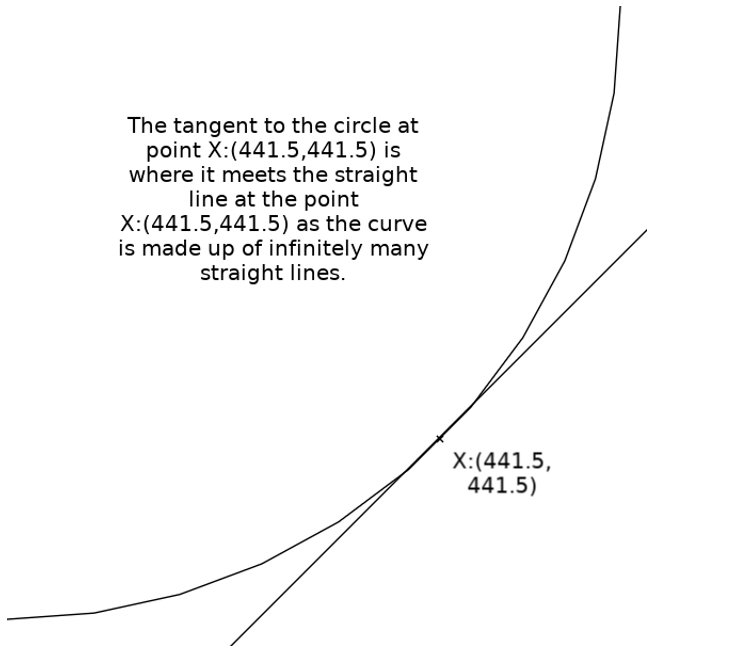
\includegraphics[scale=0.65]{Infinitesimals Simulation}\\
Q: How to define \underline{infinitesimals}?\\
$\rightarrow$ Use idea of a tangent touching a curve at a point.\\
$\rightarrow$ We interpret "touching" to mean that the curve and the tangent line \underline{intersect} in an infinitesimal piece of a curve.\\
\begin{center}
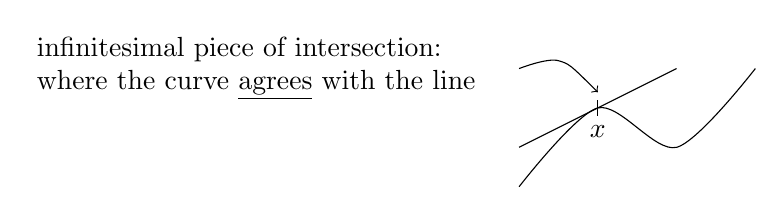
\begin{tikzpicture}
\draw plot[smooth] coordinates{(0,0)(1,1)(2,0.5)(3,1.5)};
\draw (1,1.1) -- (1,0.9) node[below]{$x$};
\draw (0,0.5) -- (2,1.5);
\draw[<-] plot[smooth] coordinates{(1,1.2)(0.5,1.6)(0,1.5)}node[text width= 6cm,left]{infinitesimal piece of intersection: where the curve \underline{agrees} with the line};
\end{tikzpicture}
\end{center}
\underline{Problem}: In general we cannot define what a tangent is except for a circle.
\begin{centering}
\begin{multicols}{2}
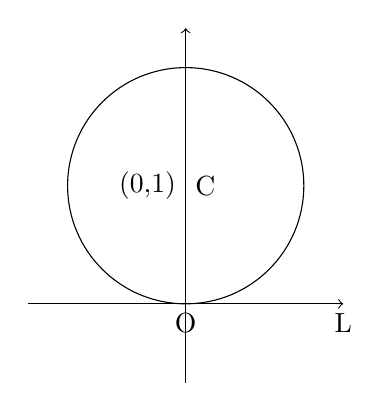
\begin{tikzpicture}
\draw (0,1.5)node[left]{(0,1)} node[right]{C} circle (1.5cm);
\draw [->] (0,-1) -- (0,0)node[below]{O} -- (0,3.5);
\draw [->] (-2,0) -- (2,0)node[below]{L};
\end{tikzpicture}\\
when a line intersects a circle at exactly \underline{one} point, then it's a tangent to the circle\\
$\rightsquigarrow$ calculate the intersection of the circle, C, and a line, L.\\
$\rightarrow$ we use a coordinate system
$C: x^2 + (y-1)^2 - 1 = 0$\\
$L: y=0 $
\end{multicols}
$(nL = \{(x,0) | x^2 = 0\})$\\
\end{centering}
$\rightarrow$ to have more than the point (0,0), we do not allow to conclude $x^2=0 \rightarrow x=0!$\\
\underline{Definition}: (First-order) infinitesimals are $d \leftarrow R$ such that $d^2=0$\\
$D:=\{$do$ R|d^2=0\}$\\
Q: What is R?
\begin{itemize}
\item[$\rightarrow$] It is \underline{not} $\mathbb{R}$ (the real numbers) because $x^2=0 \rightarrow x=0$ for $x \leftarrow \mathbb{R}$
\item[$\rightarrow$] We want R to have the properties similar to $\mathbb{R}$:
\begin{enumerate}
\item I have addition and subtraction
\item I have multiplication
\item $\mathbb{Q} c R$ (in fact $\mathbb{R} c R $)
$\rightarrow$ rational numbers: numbers that can be written as fractions.\\
\end{enumerate}
\underline{Intuition:} R is an extension of the reals by adding \underline{all} the missing infinitesimals.\\
\underline{Caution} you cannot divide freely by numbers in R\\
Suppose d $\leftarrow$ D has an inverse, $d^-1$\\
${d^-1}{d} = 1$ but $d^-1\underbrace{d.d}_{\underset{d = 0}{d^2 = 0}} = d$
\end{itemize}
\end{enumerate}

\section{Q: Can infinitesimals solve the \underline{tangent problem?}}
Definition (tangent$\leftarrow$ due to Leibniz) - a tangent is a line that intersects a curve in two infinitesimally close points.
\begin{multicols}{2}
\begin{centering}
\begin{tikzpicture}
\draw[->] (-3,0) -- (3,0);
\draw[->] (0,-1.5) -- (0,3.5);
\draw[scale=0.5,domain=-2.5:2.5,smooth,variable=\x,black] plot ({\x},{\x*\x}) node[right]{$f(x)=x^2$};
\draw[dotted] (1,2) -- (1,0) node[below]{$x_0$};
\draw[dotted] (1,2) -- (0,2) node[left]{$y_0$};
\draw[-] (0.5,0) -- (1.1,2.5);
\end{tikzpicture}
\\
Using definition of Leibniz, we are looking at the secant line through $(x_0,f(x_0)),(x_0+d,f(x_0+d))$
\end{centering}
\end{multicols}
\begin{enumerate}
\item \begin{eqnarray*}
f(x_0+d) & =& (x_0+d)^2 \\
&=& {X_0}^2 + 2{x_0}d + d^2 \\
&=& {X_0}^2 + 2{x_0}d \\
&=& f(x_0) + 2{x_0}d \\
f(x_0+d) - f(x_0) &=&   2{x_0}d \\
f(x_0+d) - f(x_0) &=&  2{x_0}\cdot((x_0+d)-x_0) \\
(y_1 - y_0  &=& m(x_1 - x_0)) 
\end{eqnarray*}
$\rightsquigarrow$ $y = f(x_0) + 2{x_0}d $ is the infinitesimal piece of the tangent at $ (x_0,f(x_0)) $\\
$\rightsquigarrow$ for any $ h \leftarrow R $ we get the equation 
$y = f(x_0) + 2{x_0}h$
\begin{center}
\begin{tikzpicture}
\draw (3,3) arc(360:270:6);
\draw(-1,-4) -- (5.6,4);
\draw[dotted] (1.5,-1) -- (1.5,-4)node[left]{$x_0$};
\draw[dotted] (1.7,-0.8)node[text width= 8cm,right]{This is the infinitesimal part where\\ the line and graph $f()$ agree.} -- (1.7,-4)node[right]{$x_0+d$};
\draw[dotted] (1.5,-1) -- (-3,-1)node[below]{$f(x_0)$};
\draw[dotted] (1.5,-0.8) -- (-3,-0.8)node[above]{$f(x_0+d)$};
\end{tikzpicture}
\end{center}

\item 
$f:R\mapsto R$ $x\mapsto x^3$\\
\begin{eqnarray*}
f(x_0+d) = (x_0+d)^3 &=& (x_0+d)^2(x_0+d)\\
& = & ({x_0}^2+2{x_0}d)(x_0+d) = {x_0}^3 + 2{x_0}^2 d + {x_0}^2 d + \underbrace{2{x_0}d^2}_{0}\\
& = &{x_0}^3 + 3{x_0}^2 d \\
& = & f(x_0) + \underbrace{3{x_0}^2}_{f(x_0)}d
\end{eqnarray*}
\item
\begin{eqnarray*}
s(t) &=& ut + \frac{1}{2}gt^2\\
s(t+dt) &=& u(t+dt) + \frac{1}{2}g(t+dt)^2\\
& = & ut + udt +  \frac{1}{2}g(t^2 2tdt)\\
& = & \underbrace{ut + \frac{1}{2}gt^2}_{s(t)} + (u+gt)dt\\
\end{eqnarray*}
\\
\\
\begin{centering}
$v(t) = \dot{s(t)}= u + gt$\\
$v(t + dt) = u + g(t+dt) = \underbrace{u + gt}_{v(t)} + gdt$\\
$a(t) = \dot{v(t)} = \ddot{s(t)} = g$\\
\end{centering}
\end{enumerate}

\underline{Axiom:} (Kock-Lawvere) For each $f: D\mapsto R$ there are \underline{unique} $a,b \leftarrow R$ such that $f(d) = a +b.d$ $ Vd \leftarrow D$
\begin{multicols}{2}
\begin{tikzpicture}
\draw[->] (-3,0) -- (0,0)node[left]{D} -- (3,0);
\draw[->] (0,-1) -- (0,3);
\draw[-] (-0.2,1.4) -- (0.2,1.6);
\draw plot[smooth]
coordinates{(-1,-0.2)(-1.1,0)(-1,0.2)};
\draw plot[smooth]
coordinates{(1,-0.2)(1.1,0)(1,0.2)};
\end{tikzpicture}
(This means we model the assumption made that every curve is made of infinitesimal line segments at each point).
\end{multicols}
$f(0) = a+b.0 = a$\\
$\rightsquigarrow$ b is the gradient of the line and hence \underline{the} gradient of $f$ at $0$. (Because it is simply determined by $f$).\\
\underline{Consequence:}\\
Consider $f:R\rightarrow R$ at $x_0 \leftarrow R$\\
Define $f_{x_0} : D\rightarrow R$ $d\mapsto f(x_0 + d)$\\
By K-L we have unique $a_{x_0}, b_{x_0} \leftarrow R$ such that \\
$$f_{x_0}(d) = a_{x_0}+b_{x_0}.d =  f_{x_0}(0) + b_{x_0}.d$$\\
i.e. $$f(x_0 + d) = f(x_0) + b_{x_0}.d$$\\
\underline{Def} $f'(x_0) := b_{x_0}$ is the \underline{derivative} of $f$ at $x_0$\\
$\rightsquigarrow$ $f'(x_0)$ is the gradient of the infinitesimal line of the graph of $f$ at $(x_0,f(x_0))$, "the gradient of $f$ at $x_0$".\\

\section{Rules for Calculating Derivatives:}
\subsection{Linearity}
\begin{center}
$f,g : R \rightarrow R$, $\lambda \leftarrow R$\\
$f + \lambda : R \rightarrow R$, $ x \mapsto f(x) + \lambda g(x)$\\
$(f + \lambda)' = f' + \lambda(g')$\\
\end{center}
\underline{Example:}\\
\begin{center}
$f(x) = x^2$, $g(x) = x^3$, $\lambda = 5$\\
$(f+\lambda g)(x) = x^2 + 5x^3$\\
$f'(x) = 2x$, $g'(x) = 3x^2$\\
$(f+\lambda g)'(x) = 2x + 15x^2$\\
\end{center}

\subsection{Product Rule}
\begin{center}
$f.g: R \rightarrow R$, $x\mapsto f(x).g(x)$\\
$(f.g)' = f'.g + f.g'$\\
\end{center}
\underline{Example:}
\begin{center}
$f(x) = x$, $g(x) = x^2$\\
$(f.g)(x) = x^3$\\
$f'(x) = 1$, $g'(x) = 2x$\\
$(f.g)'(x) = 1.x^2+x.2x = 3x^2$\\
\end{center}

\subsection{Chain Rule}
\begin{center}
$f,g : R \rightarrow R$\\
$f\circ g : R \rightarrow R$ 	$x \mapsto f(g(x))$ (composition)\\
$(f\circ g)' = (f'\circ g).g'$\\
\end{center}
\underline{Examples:}\\
\begin{enumerate}
\item[1)]
\begin{center}
$f(x) = x^2, g(x) = x^3, f'(x) = 2x, g'(x) = 3x^2$\\
$(f \circ g)(x) = f(g(x)) = f(x^3) = (x^3)^2 = x^6$\\
$(f \circ g)'(x) = f'(g(x)).g'(x) = 2x(x^3).3x^2 = 2x^3.3x^2 = 6x^5$\\
\end{center}
\item[2)]
\begin{center}
$f(x) = x^2,  g(x) = 3x^5 + 2x^2 +5$\\
$(f \circ g)(x) = f(g(x)) = (3x^5+2x^2+5)^2$\\
$f'(x) = 2x, g'(x)= 3.5x^4 + 2.2x + 0 = 15x^4 + 4x$\\
$(f \circ g)'(x) = 2(3x^5 + 2x^2 + 5).(15x^4+4x)$\\
\end{center}
\end{enumerate}

\underline{Applications:}\\
\begin{enumerate}
\item[1)]
\begin{center}
$f(x) = x, g(x) = \underset{\text{take the multiplicative inverse}}{\frac{1}{x}}$\\
$ g:\underset{\text{the set of all}x \leftarrow R\text{that are invertible(}y \leftarrow R, xy = 1\text{)}}{R^x}\rightarrow R$\\
\end{center}
we want to know $g'(x)$!\\
\begin{multicols}{2}
\begin{center}
$(f.g)(x) = 1 = x.\frac{1}{x} = 1$\\
$(f.g)'(x) = 0$\\
but $(f.g)'(x) = f'(x).g(x) + g'(x).f(x)$\\
$f'(x) = 1$\\
\end{center}
we find:
\begin{eqnarray*}
0 &=& 1.g(x) + g'(x).x\\
&=& \frac{1}{x} + g'(x).x\\
\rightsquigarrow g'(x)& = &-\frac{1}{x^2}
\end{eqnarray*}
\begin{center}
\begin{tikzpicture}
\draw[->] (-1,0) -- (5,0);
\draw[->] (0,-1) -- (0,3);
\draw (0.2,3) .. controls (1,0.5).. (5,0.2);
\draw (0,3) -- (1.5,0);
\draw[dotted] (0.7,1.5) -- (0.7,0) node[below] {$x_0$};
\end{tikzpicture}
\end{center}
\end{multicols}
\item[2)]
\begin{center}
$f:R^x \rightarrow R^x, g:R^x \rightarrow R^x, x \mapsto \frac{1}{x}$\\
$\frac{1}{f} = g\circ f$\\
$(\frac{1}{f})' = (g\circ f)' \rightsquigarrow (\frac{1}{f})'(x) = (g\circ f)'(x) = g'(f(x)).f'(x) = -\frac{1}{(f(x))^2}.f'(x)$\\
\end{center}
\item[3)] Deriving \underline{inverse} functions:
\begin{multicols}{2}
\begin{center}
given a function $f:R \rightarrow R$ such that $f$ is one to one and onto then it has an inverse(for composition).\\
$f^{-1} : f^{-1} \circ f = R_{id}$(identity map)$f^{-1}(f(x)) = x$\\
$f \circ f^{-1} = R_{id}$	$f(f^{-1}(y)) = y$\\
\begin{tikzpicture}
\draw[->] (-1,0) -- (5,0);
\draw[->] (0,-1) -- (0,3);
\draw (0,0) ..controls (1,2.5).. (5,2) node[below] {$f^{-1}(x) = \sqrt{x}$};
\draw (0,0) ..controls (3,0.5).. (4,3) node[right] {$f(x) = x^2$};
\end{tikzpicture}
\end{center}
\end{multicols}
Apply chain rule to 
\begin{eqnarray*}
f^{-1} : f^{-1} \circ f &=&  R_{id}\\
(f^{-1})'(f(x)).f'(x) &=& 1\\
(f^{-1})'f(x) &=& \frac{1}{f'(x)}(\frac{1}{m} = perpendicular)
\end{eqnarray*}
or rewritten 
\begin{eqnarray*}
(f^{-1})'(y) &=& \frac{1}{f'(f^{-1}(y))}\\
y &=& f(x)\\ 
x &=& f^{-1}(f(x))\\
&=& f^{-1}(y)\\
\end{eqnarray*}
\end{enumerate}

\section{The journey so far:}
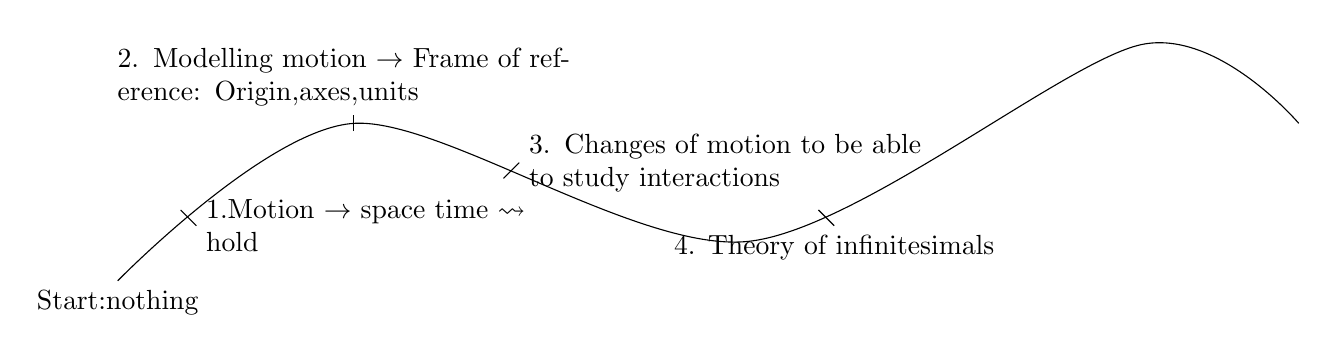
\begin{tikzpicture}
\draw plot[smooth]coordinates{(15,2)(13,3)(8,0.5)(3,2)(0,0)}node[below]{Start:nothing};
\draw (0.8, 0.9) -- (1,0.7) node[text width= 4.5cm,right]{1.Motion $\rightarrow$ space time $\rightsquigarrow$ hold};
\draw (3,1.9) -- (3,2.1) node[text width= 6cm, above]{2. Modelling motion $\rightarrow$ Frame of reference: Origin,axes,units };
\draw (4.9,1.3) -- (5.1,1.5) node[text width=5cm,right]{3. Changes of motion to be able to study interactions};
\draw (8.9,0.9) -- (9.1,0.7)node[below]{4. Theory of infinitesimals};
\end{tikzpicture}

\section{Application: Derivatives of curves}
\begin{center}
\begin{tikzpicture}
\draw[->] plot [smooth] coordinates {(0,0)(2,3)(4,1)(6,5)(7,5)(7.75,5.5)(8.5,5.25)(9,6)}node[right]{Curve $\gamma$};
\draw[->] (1,-1) node[left]{D} -- (1,0) node[left]{$\vec{e_2}$};
\draw[->] (1,-1) -- (2,-1) node[below]{$\vec{e_1}$};
\draw (1.6,4) node[right]{$\tau$} -- (3,2) node[right]{$\Delta \vec{\gamma}$} -- (4.4,0);
\draw[->] (1,-1) -- (2.7,2.3) node[left]{$\vec{\gamma}(t)$};
\draw[->] (1,-1) -- (3.4,1.2) node[below]{$\vec{\gamma}(t+dt)$};
\end{tikzpicture}
\end{center}
\begin{center}
$dt \leftarrow D$\\
\end{center}
intuition says:
\begin{itemize}
\item $\Delta \vec{\gamma}$ agrees with the curve $\gamma$.
\item a line through $\vec{\gamma}(t)$ in the direction $\vec{\gamma}$ is a \underline{tangent} at the curve $\gamma$.
\end{itemize}
\underline{Theory:}
$y:R\rightarrow R^2$, $t \mapsto \begin{bmatrix}
\gamma_1(t)\\
\gamma_2(t)
\end{bmatrix}$, $\gamma_j:R \rightarrow R$, j = 1,2 ,$
\dot{\vec{\gamma}} = 
\begin{bmatrix}
\dot{\gamma_1}(t)\\
\dot{\gamma_2}(t)\\
\end{bmatrix}$\\
\begin{center}
$\vec{\gamma}(t+dt)$ = 
$\begin{bmatrix}
\gamma_1(t+dt)\\
\gamma_2(t+dt)
\end{bmatrix}$\\
$\overset{K-L}{=}$$\begin{bmatrix}
\gamma_1(t) + \dot{\gamma_1}(t)dt\\
\gamma_2(t) + \dot{\gamma_2}(t)dt\\
\end{bmatrix}$\\
$=$ $\begin{bmatrix}
\gamma_1(t)\\
\gamma_2(t)
\end{bmatrix}$
$+$ $\begin{bmatrix}
\dot{\gamma_1}(t)\\
\dot{\gamma_2}(t)\\
\end{bmatrix}dt$\\
$= \vec{\gamma}(t) + \dot{\vec{\gamma}}(t)dt$\\
$\Delta \vec{\gamma} = \vec{\gamma}(t+dt) - \vec{\gamma}(t) = \dot{\vec{\gamma}}(t).dt \leftarrow$ \underline{Velocity}\\
$\tau: h \mapsto \gamma(t) + \dot{\gamma}(t)h$\\
\end{center}
\begin{center}
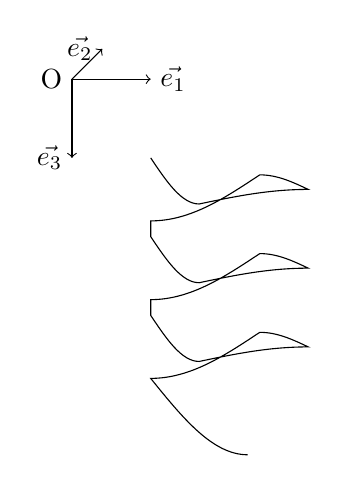
\begin{tikzpicture}
\draw[->] (0,0,0) node[left]{O} -- (0,0,-1)node[left]{$\vec{e_2}$};
\draw[->] (0,0,0) -- (1,0,0) node[right]{$\vec{e_1}$};
\draw[->] (0,0,0) -- (0,-1,0) node[left]{$\vec{e_3}$};
\draw (1,-1,0)sin(2,-1.2,1)sin(3,-1.4,0)sin(2,-1.6,-1)sin(1,-1.8,0)sin(1,-2,0)sin(2,-2.2,1)sin(3,-2.4,0)sin(2,-2.6,-1)sin(1,-2.8,0)sin(1,-3,0)sin(2,-3.2,1)sin(3,-3.4,0)sin(2,-3.6,-1)sin(1,-3.8,0)sin(3,-4,2);
\end{tikzpicture}
\end{center}
\begin{multicols}{2}
\begin{center}
From side:\\
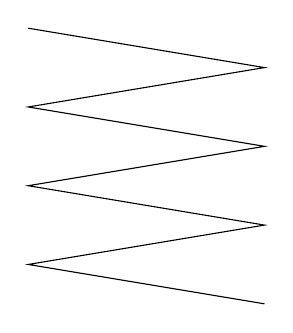
\begin{tikzpicture}
\draw (0,3.5) -- (3,3) -- (0,2.5) -- (3,2) -- (0,1.5) -- (3,1) -- (0,0.5) -- (3,0); 
\end{tikzpicture}\\
From top: looks like circular motion
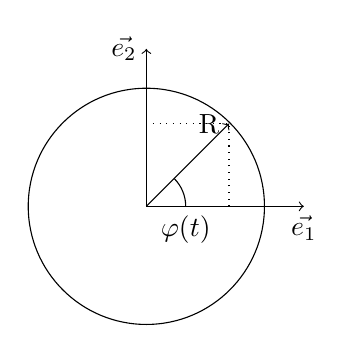
\begin{tikzpicture}
\draw (5,3) circle(1.5cm);
\draw[->] (5,3) -- (5,5) node[left]{$\vec{e_2}$};
\draw[->] (5,3) -- (7,3) node[below]{$\vec{e_1}$};
\draw[->] (5,3) -- (6.05,4.05) node[left]{R};
\draw[dotted] (6.05,3) -- (6.05,4.05);
\draw[dotted] (5,4.05) -- (6.05,4.05);
\draw (5.5,3)node[below]{$\varphi(t)$} arc (0:45:0.5);
\end{tikzpicture}\\
\end{center}
\end{multicols}
\begin{center}
$\vec{x}(t) = \begin{bmatrix}
R cos \varphi(t)\\
R sin \varphi(t)
\end{bmatrix}$\\$
\vec{x}(t) = \begin{bmatrix}
R cos \varphi(t)\\
R sin \varphi(t)\\
vt
\end{bmatrix}$\\$
\dot{\vec{x}}(t) = \begin{bmatrix}
\overset{ut}{\overbrace{-R sin \varphi(t)}}.\dot{\varphi}(t)\\
R cos \varphi(t).\dot{\varphi}(t)\\
v
\end{bmatrix}$\\$
\ddot{\vec{x}}(t) = \begin{bmatrix}
\dot{u}(t).\dot{\varphi}(t) + \dot{u}t.\ddot{\varphi}(t)\\
\\
\\
\end{bmatrix}$\\$
= \begin{bmatrix}
-R cos \varphi(t).(\dot{\varphi}(t))^2 - R sin \varphi(t).\ddot{\varphi}(t)\\
-R sin \varphi(t).(\dot{\varphi}(t))^2 + R cos \varphi(t).\ddot{\varphi}(t)\\
0\\
\end{bmatrix}$
\end{center}

\section{Physics of Motion}

\subsection{\underline{Q:}What changes motion?}
$\rightarrow$ Physical interactions.
\subsection{\underline{Q:} Why so general?}
$\rightsquigarrow$ \underline{any} form of physical interaction lead to a changes in motion.\\
$\rightarrow$ we \underline{use} changes of motion to study interactions.\\
Introduce \underline{force} as a measure of the interaction on \underline{one} object.(Reminder:
\begin{itemize}
\item[-] interaction needs at least two objects
\item[-] but we need to relate it to the change of motion of one object.)
\end{itemize}

\subsection{\underline{Q:} How to model force mathematically?}
First observation:
\begin{enumerate}
\item Has magnitude (measure of the strength of the interaction)
\item Has a direction
\end{enumerate}
$\rightsquigarrow$ model force with a vector.\\
But! (problems)\\
$\rightarrow$ It matters \underline{where} the force acts on an object. \underline{3 effects of forces:}
\begin{enumerate}
\item linear motion
\item rotation
\item deformation
\end{enumerate}
$\rightarrow$ This is \underline{not} captured by a vector.
\begin{center}
$\rightsquigarrow \vec{a}(\vec{F}) = ?$
\end{center}
\underline{Simplest} relationship:
\begin{center}
$\vec{a} \propto \vec{F} \checkmark$ (Experiment)
\end{center}
\underline{Define} Inertial mass of an object as the constant of proportionality.
\begin{itemize}
\item[-] Inertia measures how much an object resists motion
\item[-] Mass $>0$
\end{itemize}
\begin{center}
$\vec{F} = \overset{\text{inertia matrix}}{\overbrace{M}} \vec{a}$ ?
\end{center}
Or more simply
\begin{center}
$\begin{bmatrix}
F_1\\
F_2\\
F_3
\end{bmatrix}
= \begin{bmatrix}
M_1a_1\\
M_2a_2\\
M_3a_3
\end{bmatrix}$\\
so $M = 
\begin{bmatrix}
M_1 & 0 & 0\\
0 & M_2 & 0\\
0 & 0 & M_3
\end{bmatrix}
\begin{bmatrix}
a_1\\
a_2\\
a_3
\end{bmatrix}$\\
\end{center}
\begin{center}
\underline{WE DO NOT OBSERVE THIS}
\end{center}
Back to the interaction:

\subsection{\underline{Q:} What is the force acting on the other object}
\begin{center}
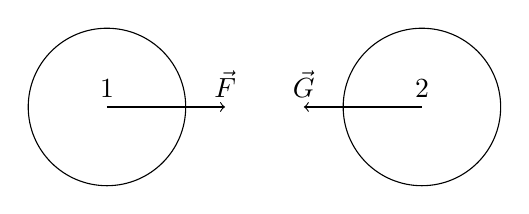
\begin{tikzpicture}
\draw (-2,0)node[above]{1} circle(1cm);
\draw (2,0)node[above]{2} circle(1cm);
\draw[->] (-2,0) -- (-0.5,0) node[above]{$\vec{F}$};
\draw[->] (2,0) -- (0.5,0) node[above]{$\vec{G}$};
\end{tikzpicture}
\end{center}
We postulate $\vec{F} = -\vec{G}$\\
$\rightarrow$ simplest assumption consistent with observation that the same objects move symmetrically after an interaction when subjected to the same initial conditions.\\
$\rightarrow$ Experiment:
\begin{center}
\begin{tikzpicture}
\draw plot[smooth] coordinates{ (0,0)(0.5,-0.1)(1,0.1)(1.5,-0.1)(2,0.1)(2.5,-0.1)(3,0.1)(3.5,-0.1)(4,0.1)(4.5,-0.1)(5,0.1)(5.5,-0.1)(6,0.1)(6.5,-0.1)(7,0.1)(7.5,-0.1)(8,0)}node[below]{river};
\draw (1,0.1)--(7,0.1)--(7,1.1)--(1,1.1)node[left]{Piece of wood}--(1,0.1);
\draw (2,1.1) -- (2,2.1);
\draw (6,1.1) -- (6,2.1);
\draw (6.5,2.1) -- (6.5,3.1) -- (5.5,3.1) -- (5.5,2.1) -- (6.5,2.1)node[right]{iron};
\draw (2.5,4) arc (90:270:1);
\draw (2.5,3.7) arc (90:270:0.7);
\draw (2.5,2) -- (2.5,2.3) -- (2.7,2.3) -- (2.7,2) -- (2.5,2);
\draw (2.5,4) -- (2.5,3.7) -- (2.7,3.7) -- (2.7,4)node[above]{magnet} -- (2.5,4);
\draw[->] (2.5,3)node[above]{$\vec{F_1}$}--(3,3);
\draw[->] (5.4,3) -- (4.9,3)node[above]{$\vec{F_2}$};
\end{tikzpicture}
\end{center}
$\rightsquigarrow$ it does not move $\rightsquigarrow \vec{F_1} = -\vec{F_2}$\\

\subsection{\underline{Q:} What is the natural state of motion?}
$\rightsquigarrow$ to be compatible with
\begin{center}
$\vec{F} = M \vec{a}$
\end{center}
We need a natural state if and only if no interaction, if and only if $\vec{F} = 0$
\begin{center}
$\Rightarrow \vec{a} = 0$    $\vec{v} = $ constant
\end{center}
a natural state has to be uniform motion with constant velocity.\\
\underline{Problems:}
\begin{enumerate}
\item Velocity is \underline{relative}(\underline{dependent} on frame of reference) but now acceleration is \underline{absolute}(\underline{independent}(not true for \underline{all} reference frames)of frame of reference).
\item I observe objects being naturally at \underline{rest!} so $\vec{v} = 0$!
\end{enumerate}
Galileo's objection to $2$:\\
$\rightarrow$ Ship argument: you cannot  \underline{tell} (with physical experiment) whether you are at rest or moving with a constant velocity. (Galileo relativity of velocity).\\
Consequence:\\
$\rightarrow$ We have to explain why things are at rest despite force acting $\rightsquigarrow$(balanced forces).\\
$\rightarrow$ this makes our explanations more complicated.\\
But: can explain celestial and terrestrial motion in one theory.\\

\section{Physics of Motion}
\begin{enumerate}
\item Interaction $\rightsquigarrow$ changes of motion(state:velocity,change:acceleration) $\rightsquigarrow$ acceleration.
\item Interaction 
\begin{center}
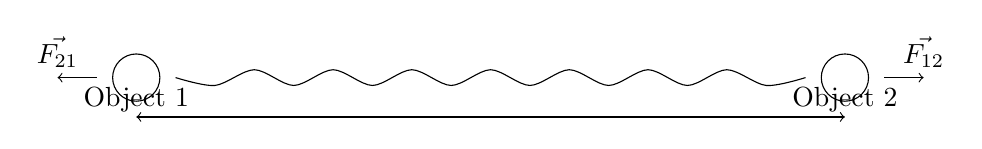
\begin{tikzpicture}
\draw plot[smooth] coordinates{ (-4,0)(-3.5,-0.1)(-3,0.1)(-2.5,-0.1)(-2,0.1)(-1.5,-0.1)(-1,0.1)(-0.5,-0.1)(0,0.1)(0.5,-0.1)(1,0.1)(1.5,-0.1)(2,0.1)(2.5,-0.1)(3,0.1)(3.5,-0.1)(4,0)};
\draw (-4.5,0) circle(0.3cm)node[below]{Object 1};
\draw (4.5,0) circle(0.3cm)node[below]{Object 2};
\draw [<->] (-4.5,-0.5) -- (4.5,-0.5);
\draw [->] (-5,0) -- (-5.5,0) node[above]{$\vec{F_{21}}$};
\draw [->] (5,0) -- (5.5,0) node[above]{$\vec{F_{12}}$};
\end{tikzpicture}
\end{center}
break down interaction into 2 parts, individual to each object.
\item Mathematical model of force?\\
\underline{Observe:}
\begin{itemize}
\item[-] magnitude(strength of interaction)
\item[-] directions
\end{itemize}
\underline{First guess} - vector model $\rightsquigarrow$ needs more justification!\\
Experiments with springs to test vector character $\checkmark$
\item Guess physical laws of forces
\begin{itemize}
\item Newton's 3rd law:$\vec{F_{12}} = -\vec{F_{21}}$
Experiment: Magnet on a boat $\checkmark$.
\item Link force and acceleration:
\begin{center}
$\rightarrow \vec{F} \parallel \vec{a}$\\$
\rightarrow |\vec{F}| \uparrow \Rightarrow |\vec{a}|\uparrow$\\(constraints from observations)
\end{center}
\item Simplest link:
\begin{center}
$\vec{a} = k\vec{F}$  $k>0$ 
\end{center}
(but also \underline{others} that need to be refuted by experiments).\\
Experiment:$\checkmark$ - e.g. ball rolling down a ramp\\
define $m = \frac{1}{k}$ (inertial mass)\\
(Physics of inertia?!)
\begin{center}
$\vec{F} = m\vec{a}$
\end{center}
\underline{Problem!} \begin{itemize}
\item [-] $\vec{F}$ (interaction) is absolute.
\item [-] $\vec{a}$ (acceleration) is relative to frame of reference.
\end{itemize}
\underline{Q:} Is there accelerated motion without a force?\\
$\rightarrow$ \underline{No} for \underline{point-particles}?$\leftarrow$ justify!\\
\underline{Newton's 1st Law:} $\vec{F} = 0 \Rightarrow \vec{a} = 0 \Rightarrow \vec{v} = $ constant (law of inertia).\\
For Newton's first law to hold you need a special frame of reference (inertial frame of reference where the law of inertia holds).\\
Experiment: Foucault has shown that the Earth is \underline{not} inertial.\\
\newpage
\begin{center}
\underline{Problem}
\begin{multicols}{2}
\underline{Absolutist interpretation:}
(Newton)
\begin{itemize}
\item [$\rightarrow$] there is absolute space and absolute time.
\item [$\rightarrow$] acceleration has to be taken as relative to absolute space.
\end{itemize}
\vfill\null
\columnbreak
\underline{Relativist interpretation:}
(dominating today due to Einstein)
\begin{itemize}
\item [$\rightarrow$] there is at least one(and infinitely many) inertial forms of reference.
\item [$\rightarrow$] Newton's laws are only valid in an inertial reference frame. 
\end{itemize}
\end{multicols}
\end{center}
\end{itemize}
\end{enumerate}
\end{document}